% ═══════════════════════════════════════════════════════════════════════════
%  DDF — préambule commun aux sept articles.  % ═══════════════════════════════════════════════════════════════════════════
%  DDF — préambule commun aux sept articles.  % ═══════════════════════════════════════════════════════════════════════════
%  DDF — préambule commun aux sept articles.  \input{ddf-common} en tête.
%  Définit : la mise en page, les macros, le bloc de série, la déclaration
%  d'usage d'outils, et le bloc de traçabilité.
% ═══════════════════════════════════════════════════════════════════════════
\documentclass[11pt,a4paper]{article}
\usepackage[margin=2.3cm]{geometry}
\usepackage{amsmath,amssymb,booktabs,hyperref,graphicx,xcolor}
\usepackage[expansion=false]{microtype}
\hypersetup{colorlinks=true,linkcolor=blue!45!black,citecolor=blue!45!black,urlcolor=blue!45!black}

% ---------- macros physiques ----------
\newcommand{\MPl}{M_{\rm Pl}}\newcommand{\Mred}{\bar M_{\rm Pl}}
\newcommand{\Mfive}{M_5}\newcommand{\MS}{M_S}\newcommand{\V}{\mathcal V}
\newcommand{\Neff}{N_{\rm eff}}\newcommand{\cb}{c_b}\newcommand{\ab}{\alpha_b}

% ---------- étiquettes épistémiques ----------
\newcommand{\Derived}{\textit{[Derived]}}
\newcommand{\Input}{\textit{[Input, natural]}}
\newcommand{\Posited}{\textit{[Posited]}}
\newcommand{\Candidate}{\textit{[Candidate]}}
\newcommand{\Open}{\textit{[Open, declared]}}
\newcommand{\Verified}{\textit{[Verified]}}

% ---------- bloc de série : \seriesdate{III}{The medium} ----------
\newcommand{\seriesdate}[2]{%
 \date{\small \textit{Cosmic Shadow Geometry} \\ \small Article #1 of VII
 \,\textperiodcentered\, #2 \,\textperiodcentered\, \today}}

% ---------- déclaration d'outils, identique dans les sept ----------
\newcommand{\toolsstatement}{%
\section*{Declaration on computational tools}
\addcontentsline{toc}{section}{Declaration on computational tools}
\small
This work was carried out by the author alone, without institutional affiliation.
\textbf{Large language models were used as computational and analytical assistants
throughout}: to write and debug the numerical scripts, to run the scans and
minimisations, to produce the figures, to check algebra and dimensional
consistency, to search and summarise the literature, and to audit drafts for
internal contradictions. Several distinct systems were used and cross-checked
against one another; no single system's output was accepted without an
independent numerical or analytical verification.

\textbf{The author is solely responsible for the physical hypotheses, the
interpretation of every result, the epistemic labels attached to each claim, and
the decision of what to publish and what to withdraw.} All quantitative
statements in this paper are reproduced by the scripts listed in the
traceability section; a reader who runs them obtains the numbers printed here
without needing any language model. Where an earlier draft contained an error
introduced by an unverified computation, it is recorded as a withdrawal rather
than silently removed.
\normalsize}

% ---------- bloc de traçabilité : \traceability{V}{...} ----------
\newcommand{\traceability}[2]{%
\section*{Data availability, traceability and reproducibility}
\addcontentsline{toc}{section}{Traceability}
\small
Every number, table and figure in this paper is regenerated by the scripts of
this article's folder. The complete repository ---sources, scripts, proof files,
figures and compiled documents for all seven articles--- is at
\url{https://github.com/HBoufourou}.

\textbf{Folder \texttt{article-#1/} contains:}
\begin{itemize}\itemsep2pt
\item \texttt{tex/} --- the \LaTeX\ source and the shared preamble \texttt{ddf-common.tex};
\item \texttt{scripts/} --- every computation, each runnable standalone with
      \texttt{python3 <name>.py} and printing its own verification verdict;
\item \texttt{proofs/} --- the JSON files carrying the certified values.
      \textbf{Any number absent from \texttt{proofs/} is not certified};
\item \texttt{data/} --- the CSV tables underlying the figures;
\item \texttt{figures/} --- the PNG files, regenerated by \texttt{scripts/figures.py};
\item \texttt{pdf/} --- the compiled article;
\item \texttt{VERIFICATION.txt} --- the output of the verification suite.
\end{itemize}
#2
\normalsize}
 en tête.
%  Définit : la mise en page, les macros, le bloc de série, la déclaration
%  d'usage d'outils, et le bloc de traçabilité.
% ═══════════════════════════════════════════════════════════════════════════
\documentclass[11pt,a4paper]{article}
\usepackage[margin=2.3cm]{geometry}
\usepackage{amsmath,amssymb,booktabs,hyperref,graphicx,xcolor}
\usepackage[expansion=false]{microtype}
\hypersetup{colorlinks=true,linkcolor=blue!45!black,citecolor=blue!45!black,urlcolor=blue!45!black}

% ---------- macros physiques ----------
\newcommand{\MPl}{M_{\rm Pl}}\newcommand{\Mred}{\bar M_{\rm Pl}}
\newcommand{\Mfive}{M_5}\newcommand{\MS}{M_S}\newcommand{\V}{\mathcal V}
\newcommand{\Neff}{N_{\rm eff}}\newcommand{\cb}{c_b}\newcommand{\ab}{\alpha_b}

% ---------- étiquettes épistémiques ----------
\newcommand{\Derived}{\textit{[Derived]}}
\newcommand{\Input}{\textit{[Input, natural]}}
\newcommand{\Posited}{\textit{[Posited]}}
\newcommand{\Candidate}{\textit{[Candidate]}}
\newcommand{\Open}{\textit{[Open, declared]}}
\newcommand{\Verified}{\textit{[Verified]}}

% ---------- bloc de série : \seriesdate{III}{The medium} ----------
\newcommand{\seriesdate}[2]{%
 \date{\small \textit{Cosmic Shadow Geometry} \\ \small Article #1 of VII
 \,\textperiodcentered\, #2 \,\textperiodcentered\, \today}}

% ---------- déclaration d'outils, identique dans les sept ----------
\newcommand{\toolsstatement}{%
\section*{Declaration on computational tools}
\addcontentsline{toc}{section}{Declaration on computational tools}
\small
This work was carried out by the author alone, without institutional affiliation.
\textbf{Large language models were used as computational and analytical assistants
throughout}: to write and debug the numerical scripts, to run the scans and
minimisations, to produce the figures, to check algebra and dimensional
consistency, to search and summarise the literature, and to audit drafts for
internal contradictions. Several distinct systems were used and cross-checked
against one another; no single system's output was accepted without an
independent numerical or analytical verification.

\textbf{The author is solely responsible for the physical hypotheses, the
interpretation of every result, the epistemic labels attached to each claim, and
the decision of what to publish and what to withdraw.} All quantitative
statements in this paper are reproduced by the scripts listed in the
traceability section; a reader who runs them obtains the numbers printed here
without needing any language model. Where an earlier draft contained an error
introduced by an unverified computation, it is recorded as a withdrawal rather
than silently removed.
\normalsize}

% ---------- bloc de traçabilité : \traceability{V}{...} ----------
\newcommand{\traceability}[2]{%
\section*{Data availability, traceability and reproducibility}
\addcontentsline{toc}{section}{Traceability}
\small
Every number, table and figure in this paper is regenerated by the scripts of
this article's folder. The complete repository ---sources, scripts, proof files,
figures and compiled documents for all seven articles--- is at
\url{https://github.com/HBoufourou}.

\textbf{Folder \texttt{article-#1/} contains:}
\begin{itemize}\itemsep2pt
\item \texttt{tex/} --- the \LaTeX\ source and the shared preamble \texttt{ddf-common.tex};
\item \texttt{scripts/} --- every computation, each runnable standalone with
      \texttt{python3 <name>.py} and printing its own verification verdict;
\item \texttt{proofs/} --- the JSON files carrying the certified values.
      \textbf{Any number absent from \texttt{proofs/} is not certified};
\item \texttt{data/} --- the CSV tables underlying the figures;
\item \texttt{figures/} --- the PNG files, regenerated by \texttt{scripts/figures.py};
\item \texttt{pdf/} --- the compiled article;
\item \texttt{VERIFICATION.txt} --- the output of the verification suite.
\end{itemize}
#2
\normalsize}
 en tête.
%  Définit : la mise en page, les macros, le bloc de série, la déclaration
%  d'usage d'outils, et le bloc de traçabilité.
% ═══════════════════════════════════════════════════════════════════════════
\documentclass[11pt,a4paper]{article}
\usepackage[margin=2.3cm]{geometry}
\usepackage{amsmath,amssymb,booktabs,hyperref,graphicx,xcolor}
\usepackage[expansion=false]{microtype}
\hypersetup{colorlinks=true,linkcolor=blue!45!black,citecolor=blue!45!black,urlcolor=blue!45!black}

% ---------- macros physiques ----------
\newcommand{\MPl}{M_{\rm Pl}}\newcommand{\Mred}{\bar M_{\rm Pl}}
\newcommand{\Mfive}{M_5}\newcommand{\MS}{M_S}\newcommand{\V}{\mathcal V}
\newcommand{\Neff}{N_{\rm eff}}\newcommand{\cb}{c_b}\newcommand{\ab}{\alpha_b}

% ---------- étiquettes épistémiques ----------
\newcommand{\Derived}{\textit{[Derived]}}
\newcommand{\Input}{\textit{[Input, natural]}}
\newcommand{\Posited}{\textit{[Posited]}}
\newcommand{\Candidate}{\textit{[Candidate]}}
\newcommand{\Open}{\textit{[Open, declared]}}
\newcommand{\Verified}{\textit{[Verified]}}

% ---------- bloc de série : \seriesdate{III}{The medium} ----------
\newcommand{\seriesdate}[2]{%
 \date{\small \textit{Cosmic Shadow Geometry} \\ \small Article #1 of VII
 \,\textperiodcentered\, #2 \,\textperiodcentered\, \today}}

% ---------- déclaration d'outils, identique dans les sept ----------
\newcommand{\toolsstatement}{%
\section*{Declaration on computational tools}
\addcontentsline{toc}{section}{Declaration on computational tools}
\small
This work was carried out by the author alone, without institutional affiliation.
\textbf{Large language models were used as computational and analytical assistants
throughout}: to write and debug the numerical scripts, to run the scans and
minimisations, to produce the figures, to check algebra and dimensional
consistency, to search and summarise the literature, and to audit drafts for
internal contradictions. Several distinct systems were used and cross-checked
against one another; no single system's output was accepted without an
independent numerical or analytical verification.

\textbf{The author is solely responsible for the physical hypotheses, the
interpretation of every result, the epistemic labels attached to each claim, and
the decision of what to publish and what to withdraw.} All quantitative
statements in this paper are reproduced by the scripts listed in the
traceability section; a reader who runs them obtains the numbers printed here
without needing any language model. Where an earlier draft contained an error
introduced by an unverified computation, it is recorded as a withdrawal rather
than silently removed.
\normalsize}

% ---------- bloc de traçabilité : \traceability{V}{...} ----------
\newcommand{\traceability}[2]{%
\section*{Data availability, traceability and reproducibility}
\addcontentsline{toc}{section}{Traceability}
\small
Every number, table and figure in this paper is regenerated by the scripts of
this article's folder. The complete repository ---sources, scripts, proof files,
figures and compiled documents for all seven articles--- is at
\url{https://github.com/HBoufourou}.

\textbf{Folder \texttt{article-#1/} contains:}
\begin{itemize}\itemsep2pt
\item \texttt{tex/} --- the \LaTeX\ source and the shared preamble \texttt{ddf-common.tex};
\item \texttt{scripts/} --- every computation, each runnable standalone with
      \texttt{python3 <name>.py} and printing its own verification verdict;
\item \texttt{proofs/} --- the JSON files carrying the certified values.
      \textbf{Any number absent from \texttt{proofs/} is not certified};
\item \texttt{data/} --- the CSV tables underlying the figures;
\item \texttt{figures/} --- the PNG files, regenerated by \texttt{scripts/figures.py};
\item \texttt{pdf/} --- the compiled article;
\item \texttt{VERIFICATION.txt} --- the output of the verification suite.
\end{itemize}
#2
\normalsize}

\graphicspath{{figures/}{../figures/}}
\title{\bfseries The Dark Dimension Framework from Type I$'$ strings:\\
three norm identities, two no-go results,\\ and a candidate that reaches the window}
\author{Hicham Boufourou\\ \small Independent Researcher, Brussels, Belgium\\ \small\texttt{hicham.boufourou@hotmail.com}}
\seriesdate{V}{from Type I$'$ strings}
\begin{document}\maketitle

\begin{abstract}
the Dark Dimension Framework is a five-dimensional framework whose effective theory contains exactly one order-unity constant it cannot produce: $c_b$, the ultraviolet vertex coupling the bulk scalar to the trace of the localised stress tensor. This paper embeds the framework in Type I$'$ string theory and computes that vertex. A matching theorem first establishes that the string-side coefficient and the parent constant multiply the same operator with no residual factor. A sequential Einstein-frame reduction then gives the D8 tension-coupling vector exactly, $|\vec w|^2=6$, confirmed against published disc amplitudes; the same counting applied to the massive-IIA flux term and to the domain-wall tension gives $|\vec v|^2=14$ and $|\vec u|^2=24$, with integer inner products $\vec w\cdot\vec v=8$, $\vec w\cdot\vec u=11$. The bound $c_b\leq\sqrt{255/56}$ excludes two of the parent's four coupling benchmarks. Explicit vacua follow: a Large Volume minimum at realistic topology reproduces the parent's scale to three percent of its own node and gives $c_b=7\sqrt6/12$ (vanilla) and $\sqrt{5/6}$ (fibred); the domain-wall route gives $11\sqrt6/12$. All exceed the parent window $[0.30,0.61]$, and the boundary weight $w_1$ that could have moved that window has been audited and confirmed. Two autonomous no-go results are established: five independent pinning mechanisms fail by sixteen to forty-seven orders, and massive IIA is incompatible with a mesoscopic interval. The resolution is that the Dark Dimension Framework requires a \emph{mixed} light state, which needs two flat directions --- available for $h^{1,1}\geq4$, and, once the D-term levy is budgeted, for $h^{1,1}=5$. An explicit candidate is exhibited --- polytope 3181 of the orientifold database, $h^{1,1}=5$, $h^{2,1}=81$, $\chi=-152$, identified by its six-divisor signature and not by any catalogue index. It passes every computable test, its projections are invariant over twelve orders of volume, and the K3 wrapping gives $|\vec p|=0.4514$ at the centre of the window at the reference point. \textbf{The candidate is not unique}: a scan of $56\,714$ triangulations finds sixteen further polytopes with the same structure, and on the three sharing its Hodge numbers the window is reached in $13$--$17\%$ of admissible points. Imposing the Large-Volume hierarchy on the enumerated family then splits it cleanly: nine geometries with a proper fibration carry median couplings in $[0.30,0.58]$, eleven without carry medians above $0.67$, and the two groups do not overlap. \textbf{Reaching the window is therefore a property of a subclass selected by the fibration, not of one member} --- but the position along the flat directions is not fixed on any member, and this paper does not claim it is. The last step --- fixing the position along the flat directions --- requires string-loop coefficients that are not computable for a general Calabi--Yau, and applying the published functional form for this class shows the minimum tending to the boundary of the K\"ahler cone. The coupling is therefore not fixed. What survives is an angle-independent sum rule: the two light states are experimentally indistinguishable, so the fifth-force observable is $\alpha_b^2+\alpha_b'^2=2w_1|\vec p|^2$, which requires no loop coefficient at all.
\end{abstract}

\section{The gap, and the matching theorem}
the Dark Dimension Framework proposes that dark matter, dark energy and the radial-acceleration relation are three readings of one structure: an $8.2\,\mu$m interval carrying gravity and one dark scalar, with the Standard Model on a thin core at one boundary~\cite{DDF1,DDF2,DDF3,DDF4}. Its interaction with matter is written once, covariantly,
\begin{equation}
S_{\rm int}=-\frac{c_b}{M_5^{3/2}}\int d^5x\,\sqrt{-g_5}\;\delta(y-y_0)\,\Phi\,g_{\mu\nu}T^{\mu\nu}_b,
\qquad \alpha_b=c_b\sqrt{2w_1}.
\end{equation}
The thin core makes the overlap unity to twenty-six decimal places, so no form factor remains: $c_b$ \emph{is} the ultraviolet vertex, and an effective theory cannot produce it.

\paragraph{Matching.} Reducing the parent operator on mode $n$ gives $c_b\psi_n(y_0)/M_5^{3/2}$; with the parent's boundary weight $w_n\equiv\pi R|\psi_n(y_0)|^2$ and its own calibration $\bar M_{\rm Pl}^2=M_5^3(\pi R)$ --- whose quoted numbers confirm the \emph{reduced} Planck mass --- this is $c_b\sqrt{w_n}\,\varphi_nT^\mu_{\ \mu}/\bar M_{\rm Pl}$. For a flat zero mode $w=1$, so the parent's constant and our tree coefficient multiply the same operator, with no residual factor. The factorisation $\alpha_b=c_b\sqrt{2w_1}$ is precisely the junction.

\section{Family selection}
Ho\v{r}ava--Witten reproduces the geometry natively but is excluded as the dark dimension: proton stability bounds its interval twenty orders below target, and warping worsens it~\cite{ReigRuiz}. The same analysis designates the survivors --- non-unified D-brane models --- and Type I$'$ is where three things coincide: the interval is the geometry by construction; \textbf{RR tadpole cancellation is the framework's Gauss law}, the equal and opposite boundary sources becoming a consistency condition of the string; and disc amplitudes exist. Three survival tests pass: stellar cooling for one extra dimension is weaker than the laboratory frontier~\cite{Hardy}; proton stability is safe for a non-unified $U(1)_B$~\cite{Aldazabal}; and $M_s=M_5g_s^{2/3}=0.8$--$3.6\times10^8$~GeV is consistent.

\section{Three norm identities}
Reducing $10\to9$ on the interval and $9\to4$ on $X_5$ with the Einstein and canonicity conditions gives $\alpha_1=1/4\sqrt7$, $\beta_1=-\sqrt7/4$, $\alpha_2=\sqrt{5/28}$, $\beta_2=-1/\sqrt{35}$, with $7\alpha_1+\beta_1=0$ and $2\alpha_2+5\beta_2=0$ exactly. The D8 DBI term carries $e^{(p-3)\phi/4}$ and geometric weights $9\alpha_1$, $4\alpha_2+5\beta_2$; the massive-IIA term $\tfrac12e^{5\phi/2}F_0^2$ has dilaton weight $5/2$ and, being a bulk term, also the interval factor $e^{\beta_1\rho}$; and the domain-wall tension follows from the parent's one-scale wall, $T=m_\chi^4$ with $m_\chi=M_S$, $M_S^2=m_{3/2}\bar M_{\rm Pl}$, hence $T\propto\mathcal V^{-2}$. Canonical normalisation multiplies all weights by $\sqrt2$:
\begin{equation}
\vec w=(1.7678,\,1.1952,\,1.2027),\quad
\vec v=(3.5355,\,1.1952,\,0.2673),\quad
\vec u=(4.2426,\,2.3905,\,0.5345),
\end{equation}
\begin{equation}
\boxed{\;|\vec w|^2=6,\qquad|\vec v|^2=14,\qquad|\vec u|^2=24,\qquad \vec w\cdot\vec v=8,\qquad \vec w\cdot\vec u=11.\;}
\end{equation}
Three integer norms and two integer inner products, none adjusted, all from the same exponent counting; the angles are $29.21^\circ$ and $23.56^\circ$. The dilaton entry of $\vec w$ matches the disc-amplitude coefficient $(p-3)/2\sqrt2$ of Garousi--Myers~\cite{GM} \emph{as an identity in $p$}. One inference is declared: our $\sqrt2$ arises from 4D canonical normalisation and theirs from the 10D dilaton convention. Two of these numbers are inherited rather than new. $|\vec v|^2=14$ is the four-dimensional image of the $\Delta=4$ invariant of the Romans mass under untruncated Kaluza--Klein reduction (L\"u--Pope--Stelle lineage, hep-th/9605082, hep-th/9508042); and the (dilaton, overall-volume) content of $\vec w$ reproduces the standard two-modulus scaling $V_{\rm D8}\propto\tau^{-3}\rho$ (Wrase--Zagermann, arXiv:1003.0029; lineage of Hertzberg--Kachru--Taylor--Tegmark, arXiv:0711.2512), of squared norm $31/6$. What the present reduction adds is the third axis: separating the interval length from the overall volume contributes an orthogonal $5/6$, and $|\vec w|^2=31/6+5/6=6$ exactly. The boundary term escapes the bulk $\Delta$-invariance (its transported invariant would be $\Delta=0$, no BPS value), which is why this norm appears in no $\Delta$ table. The same counting gives $|\vec w(p)|^2=(p-3)^2/5-(p-3)+6$ for a D$p$ transverse to the interval wrapping a $(p-3)$-cycle: the value $6$ is attained at $p=8$ and $p=3$ only. A dated search log accompanies this deposit; the decomposition is offered with its ancestors cited, for correction rather than as a priority claim.

\paragraph{The bound.} Since $\Phi$ is a unit vector, $c_b=|\hat n\cdot\vec w|\leq|\vec w|$; excluding the interval direction tightens this to $c_b\leq\sqrt{255/56}=2.1339$, so \textbf{the parent's benchmarks $3.02$ and $155$ are excluded} and the surviving branch is the one galactic phenomenology already preferred. The window maps to $\theta\in[73.4^\circ,81.9^\circ]$, a $12$--$25\%$ admixture of the tension direction, and --- in the (dilaton, volume) plane --- to a \emph{bimodal} composition, $p_{\rm vol}\in[0.402,0.549]\cup[0.808,0.910]$. The radion's tree Yukawa follows as $\alpha_\rho=81/28$.

\section{What $\Phi$ is, and what its mass bounds}
Reducing on $X_5$ \emph{alone} yields a five-dimensional field on the interval whose $y$-zero-mode is the modulus and whose ground state in the $y$-dependent background is the parent's bound state: two storeys of one field. The ten-dimensional identity fixes the vertex; the well fixes the profile. The two mass sources add in quadrature, $m_n^2=m_0^2+E_n^2$, so the validated tower ratios bound the uniform soft mass, $m_0<0.23\,\varepsilon=5.4$~meV; since no-scale structure protects the volume modulus but not the dilaton, this becomes a cross-exclusion between $M_S$ and the composition of $\Phi$ (dilaton fraction below $69\%$, $5\%$, $2\%$ at $M_S=4,7.6,10$~TeV).

\paragraph{Parity.} No homogeneous boundary condition on the finite interval reproduces the validated tower ratios $2.294,3.190,4.031$ (Neumann--Dirichlet gives $3.235,5.330,8.266$; Neumann--Neumann $3.134,4.501,6.734$; Dirichlet--Dirichlet $1.838,2.908,4.398$); the $|y|$ well on the covering space with both parities interleaved gives $2.295,3.188,4.013$, the fourth ratio deviating exactly where the far wall is first reached ($E_4=4.09$ against $u=4.43$). $\Phi$ is therefore not $\mathbb Z_2$-projected. The audit also confirms $w_1=5.5$ on three independently obtained numbers, so the window numbers stand.

\section{Explicit vacua, and the pattern}
\subsection{A reference Large Volume minimum}
With $\hat\xi=\xi/g_s^{3/2}$ and $\tau_s^{3/2}=\hat\xi/2$, the scale is carried by $a_s\tau_s\simeq\ln(\bar M_{\rm Pl}/m_{3/2})\simeq66$, not by $\xi$ --- which is topology. Audited minima (logarithmic gradient $\sim10^{-5}$, both eigenvalues positive):
\begin{center}\small
\begin{tabular}{cccccc}\toprule
$N$&$g_s$&$\xi$&$|\chi|$&$\mathcal V$&$m_{3/2}$\\\midrule
2&0.010&0.194&80&$1.25\times10^{20}$&25.7~meV\\
2&0.020&0.548&226&$1.23\times10^{20}$&25.7~meV\\
3&0.020&1.008&416&$4.52\times10^{20}$&14.0~meV\\\bottomrule
\end{tabular}
\end{center}
The first corresponds to $M_S=7.9$~TeV, within three percent of the parent's own node. We declare the price: $d\ln m_{3/2}/d\ln g_s=+66.7$, so the meV scale requires $g_s$ known to $\sim10^{-3}$; $g_s$ is flux-fixed and discrete, but this is a strong constraint on the vacuum.

\paragraph{A quantum-gravity check the vacuum passes.} The reference minimum satisfies the domain wall bound recently derived from the ten-dimensional supergravity equations of motion~\cite{CPV}, $\Lambda_{\rm UV}^{3}\leq M_{\rm Pl}^{2}/L_{\rm AdS}$, which simultaneously realises the gravitino conjecture and the anti-de Sitter distance conjecture. With $m_{\rm KK}=g_s/\mathcal V^{2/3}=959$~GeV and $|V_{\rm AdS}|\simeq m_{3/2}^{3}M_{\rm Pl}$ one finds $m_{\rm KK}^{3}L_{\rm AdS}=3.2\times10^{-3}<1$, and the associated lower bound on the gravitino mass holds with a margin of a factor $15$ at the string-scale cutoff. \textbf{This is not automatic.} The same bound is violated by twenty to ninety-seven orders of magnitude by KKLT-type constructions with exponentially small cosmological constant, while classical flux vacua and the Large Volume Scenario are found to comply~\cite{CPV}. The choice of LVS made here on scale grounds --- the meV window --- is therefore also the one that survives an independently derived quantum-gravity constraint, and the margin is small enough that the check had a genuine chance of failing.

\subsection{Four derived couplings, and a negative theorem}
In vanilla LVS the lightest state is the overall volume, $c_b=7\sqrt6/12=1.429$. In the fibred case the fibre direction is \emph{exactly} flat for the LVS potential --- with $\mathcal V=e^{v/2+w}$ and constant K\"ahler metric ${\rm diag}(1/2,1)$, the direction $(2,-1)$ gives $\delta\ln\mathcal V=0$ --- so it is lifted only by loops, its minimum is analytic ($\tau_f\sim\mathcal V^{2/3}$), and $m_F^2/m_{\mathcal V}^2\sim10^{-12}$ makes the light state pure fibre: $c_b=\sqrt{5/6}=0.913$. The domain wall, being the sole source once the string-scale tensions cancel, gives a rank-one matrix along $\vec u$ and $c_b=11\sqrt6/12=2.245$ with no free parameter.
\begin{center}\small
\begin{tabular}{lcc}\toprule
construction & $c_b$ & $\alpha_b=c_b\sqrt{2w_1}$\\\midrule
fibred LVS (pure fibre)&$\sqrt{5/6}=0.913$&3.03\\
vanilla LVS (overall volume)&$7\sqrt6/12=1.429$&4.74\\
domain wall&$11\sqrt6/12=2.245$&7.45\\
variant $\vec w+\vec u$&$17\sqrt{13}/26=2.358$&7.82\\
source aligned on $\vec w$&$\sqrt6=2.449$&8.12\\\bottomrule
\end{tabular}
\end{center}
\begin{figure}[h]\centering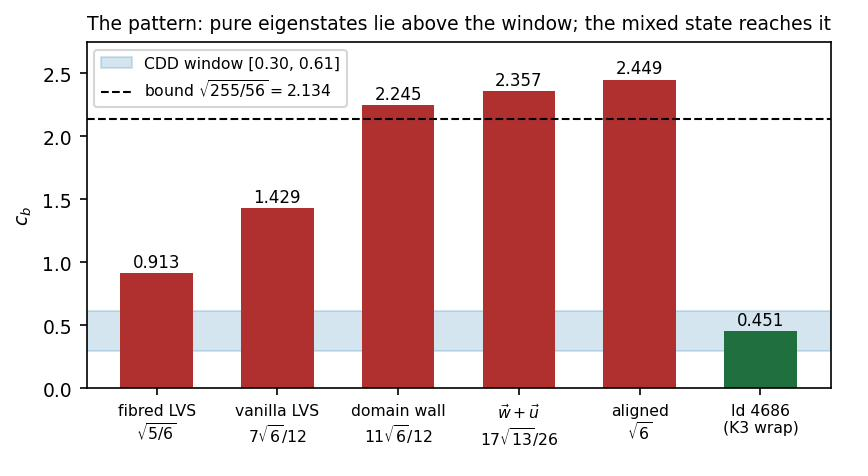
\includegraphics[width=.80\textwidth]{fig1_motif.png}
\caption{Every derived pure-eigenstate coupling lies above the phenomenological window; the mixed state of the candidate vacuum reaches it, at the reference point in the K\"ahler cone.}\end{figure}
\textbf{Every route gives $c_b\geq0.91$; the parent window lies below all of them.} The one escape --- an order-unity error in $w_1$ --- is closed by the audit above: reconciliation would require $w_1\simeq0.40$, a factor $13.5$ below the audited value, meaning a wavefunction that barely touches the brane. Hence
\begin{quote}\emph{No construction whose light state is a pure eigenstate of the moduli sector satisfies the angular condition; the window requires a mixed state.}\end{quote}

\subsection{Two autonomous no-go results}
A crossing where the volume and fibre masses meet exists at $\tau_f^*\simeq\sqrt{2A\mathcal V}$, and there the antisymmetric branch gives $c_b=0.365$, inside the window --- but reaching it requires pinning $\tau_f$ away from its loop minimum, and \textbf{five independent mechanisms fail}: D-terms by 47 orders, magnetic fluxes by 35, electric fluxes by vanishing curvature, charged matter by the wrong sign, the loop $C$-term by 16. The cause is structural: the demand was degeneracy between masses generated by mechanisms of different order in $g_s$ and $\mathcal V$.

Second, tadpole cancellation fixes the flux-to-tension ratio with no freedom: $\kappa^2T_8=g_s/4\pi\ell_s$ gives $r=c^2g_s^2R/2\ell_s\sim10^{12}$--$10^{15}$ against a target $[0.149,0.419]$, and $F_0$ is quantised so the only smaller value is zero. \textbf{Massive IIA and a mesoscopic interval are incompatible} --- the interval is $\sim10^{19}$ string lengths, and any non-zero Romans mass deposits a colossal vacuum energy across it. \emph{What $F_0=0$ then imposes:} the enclosed charge vanishes, so the tadpole cancels locally and each boundary carries eight D8s and one O8, including the far one. The parent's prediction of an empty far wall survives in its own terms (no Standard-Model matter), but eight D8-branes constitute a hidden gauge sector, and the embedding hands the framework a new judge: that sector must fit the parent's radiation budget, $\Delta N_{\rm eff}<0.3$ today and $<0.06$ under CMB-S4.

\section{The open route: mixed states}
The no-go closes a door the parent never asked to open. We had silently assumed \emph{that $\Phi$ is the lightest eigenstate of the moduli potential} --- nowhere in the Dark Dimension Framework, and contradicted by its own $m_n^2=m_0^2+E_n^2$. In the reference vacuum the soft masses are $2.2\times10^{-9}$ and $2.2\times10^{-15}$~meV against a well of $24$~meV: at the scale where the mass is generated the directions are degenerate to one part in $10^{11}$. The quasi-degeneracy never needed constructing.

For $h^{1,1}>2$ the LVS procedure leaves $h^{1,1}-2$ flat directions, all lifted by the same subleading effect, hence degenerate by construction. With two of them the light state is $\hat n=\cos t\,\hat n_1+\sin t\,\hat n_2$ and $c_b=|\cos t\,p_1+\sin t\,p_2|$ sweeps $[0,\sqrt{p_1^2+p_2^2}]$: \textbf{the window becomes accessible}. Two conditions follow. \emph{(i)} The D-term levy: chiral matter brings an anomalous $U(1)$ whose moduli-dependent FI term fixes one modulus, so $h^{1,1}=4$ leaves only one flat direction; $h^{1,1}=5$ budgets the levy, $5-2-1=2$. Alternatively --- and at no cost here --- the Dark Dimension Framework's chirality comes from the domain-wall zero modes, not from D-branes, so a non-chiral brane sector is available and no D-term arises. \emph{(ii)} The wrapping must be asymmetric: if the brane wraps the flat-subspace cycles with equal weights its vector is parallel to the volume direction, $p_1=p_2=0$, and the window is unreachable for any Calabi--Yau. This is a condition on the brane configuration, not on the topology.

\section{An explicit candidate}
\paragraph{Two calculations, and how they relate.} This section reports two computations that a reader must not conflate. \emph{The reference calculation} (the reference vacuum, its cone and its projections below) was performed on the intersection numbers first supplied for the candidate, in the divisor basis $[1,5,6,7,8]$ of that dataset, at the Large-Volume point, with one del Pezzo and the Wilson divisor fixed; it produced $|\vec p|=0.4514$ and the cone slice of Fig.~2, and every subsequent number in Articles~VI and VII descends from it. \emph{The family calculation} (the paragraph on the family below) was performed later, directly on the orientifold database, in a basis built from the K3 fibre and \emph{both} diagonal del Pezzo divisors, with both fixed; it produced the $13$--$17\%$ genericities and the class statistics of the Routes section. \textbf{The two agree on what matters --- the window is reached, at comparable genericity --- and differ in basis and in what is held fixed, so their individual values are not to be compared digit for digit.} We say this once, here, so that it need not be repeated at every number below.


The class is enumerated: a scan of $100\,354$ Calabi--Yau geometries with $1\leq h^{1,1}\leq6$ finds \textbf{exactly $61$} that are K3-fibred with two diagonal del Pezzo divisors and a Wilson divisor --- two at $h^{1,1}=4$, fourteen at $h^{1,1}=5$, forty-five at $h^{1,1}=6$~\cite{Shukla}. The fourteen at $h^{1,1}=5$ carry the polytope identifiers $2579$, $2580$, $2583$, $3352$, $4429$, $4686$, $4687$, $4689$, $5087$, $5789$, $6427$, $6430$. \textbf{The search space is finite and listed.} We have since scanned it: of $56\,714$ triangulations in the $h^{1,1}=5$ database, $128$ carry the complete structure. \textbf{Polytope 3181 reproduces the six-divisor signature exactly} --- two diagonal dP7 divisors, one K3 fibre and three Wilson divisors --- and is the identification of the candidate used here, obtained without reference to any catalogue index. \textbf{Sixteen further polytopes carry the same structure at different Hodge numbers, so the candidate is not unique}: it is one member of an enumerated family, with diagonal del Pezzo degrees ranging over $0,1,6,7,8$. We take polytope 3181 --- the entry that Shukla's catalogue lists as Id 4686 --- ($h^{1,1}=5$, $h^{2,1}=81$, $\chi=-152$), which passes every computable test. \textbf{In the basis of the reference dataset}, $[1,5,6,7,8]$, the divisors are classified by the self-intersection $\kappa_0=\kappa_{sss}$ and the degree $\Pi$ (in the database's own numbering the same content reads: K3 at divisor 1, the two dP7 at 3 and 4, Wilson at 7, 8, 9 --- see Article~VI, Fig.~1):
\begin{center}\small
\begin{tabular}{lccccl}\toprule
basis divisor & type & $\kappa_0$ & $\Pi$ & $\chi_h$ & role\\\midrule
prime 1&K3&0&24&2&fibre\\
prime 5&dP7&2&8&1&LVS ($\tau_s$)\\
prime 6&dP7&2&8&1&flat direction\\
prime 7&Wilson&$-2$&4&0&D-term\\
prime 8&Wilson&$-2$&4&0&wrapping\\\bottomrule
\end{tabular}
\end{center}
Both dP7 divisors are \emph{diagonal} ($\kappa_{sij}=0$ for $(i,j)\neq(s,s)$), so instantons generate the barrier and no runaway occurs. The volume polynomial is $\mathcal V=2t_0t_3t_4+\tfrac13t_1^3-t_1^2t_3+t_1t_3^2+\tfrac13t_2^3-t_2^2t_4+t_2t_4^2-\tfrac13t_3^3-t_3^2t_4-\tfrac13t_4^3$, giving $\tau_1=(t_1-t_3)^2$ and $\tau_2=(t_2-t_4)^2$; at the stretched-cone tip $[6,1,2,2,3]$ one finds $\mathcal V=59.33$, $\vec\tau=(12,1,1,23,19)$. The orientifold criterion is satisfied for both involutions: $\sigma_7$ has six real O3 loci and $Q_{D3}=2$, $\sigma_8$ has fourteen and $Q_{D3}=4$, both integers.

\paragraph{The cone constrains the physics.} In the $(t_2,t_4)$ plane the K\"ahler cone is a parallelogram with $t_4\in[54.34,121.77]$ and $t_2\in[t_4-54.34,\,t_4]$, on the branch $t_1-t_3<0$ --- which is essential and was the source of one erroneous verdict in this work. \textbf{A first physical consequence: the natural choice $\tau_W/\mathcal V^{2/3}=0.5$ is incompatible with the cone}, since $t_4\geq t_3$ forces this ratio above $1.5$; the value $1.512$ realised at the tip is used throughout. Numerically, writing $\delta=t_3-t_1=\sqrt{r_s}\,\mathcal V^{1/3}$ satisfies $\tau_s$ analytically and reduces the system to two unknowns, removing the catastrophic cancellation that $\tau_1=(t_1-t_3)^2$ otherwise produces. At the LVS point the metric in the \emph{four-cycle} basis, $G_{ij}=-(M^{-1})_{ij}/\mathcal V+t^it^j/2\mathcal V^2$ with $M_{ij}=\kappa_{ijk}t^k$ (the factor $\tfrac12$ matters), has eigenvalues $(2.8,3.4,22,27)\times10^{-9}$ and $5.0\times10^{-4}$ --- positive definite, condition number $1.8\times10^5$ --- and the orthogonal complement has rank two, obtained by SVD in the $G$-orthonormal frame rather than by Gram--Schmidt, which miscounts at this conditioning. The projections are then
\begin{center}\small
\begin{tabular}{lccccc}\toprule
wrapping & $p_1$ & $p_2$ & $|\vec p|$ & reachable fraction\\\midrule
\textbf{K3 (prime 1)}&$+0.0524$&$-0.4483$&$\mathbf{0.4514}$&$\mathbf{53.7\%}$\\
dP7 flat (prime 6)&$+1.2743$&$+1.0534$&1.6534&12.4\%\\
Wilson (prime 8)&$-1.4677$&$+0.8180$&1.6803&12.2\%\\
Wilson D-term (prime 7)&---&---&0.1760&0\%\\\bottomrule
\end{tabular}
\end{center}
\paragraph{The winning wrapping is the distinguished divisor.} $D_0$ is not one option among five: the checks $\kappa_{00j}=0$ for all $j$ and $c_2\!\cdot\!D_0=24$ identify it as the \emph{K3 fibre class}. The two dP7s are vertical ($\kappa_{01j}=\kappa_{02j}=0$), so the LVS blow-up and the flat direction are components of degenerate fibres; $D_3$ and $D_4$ are horizontal, their restrictions generating the fibre Picard lattice, of rank two and intersection form $\left(\begin{smallmatrix}0&2\\2&0\end{smallmatrix}\right)$. The wrapping that lands in the window is therefore the one the fibration singles out --- a naturality statement, not a selection after the fact. The fibre class is also fixed by the orientifold involution, hence even, on precisely the two triangulations on which it is a strict K3 --- a fact used in Article~VI. Being K3-fibred, the manifold also admits a heterotic dual on $K3\times T^2$, whose count matches: $n_V=h^{1,1}=5$ gives $S,T,U$ plus exactly two Wilson lines, and the geometry carries exactly two horizontal Wilson divisors; $n_H=h^{2,1}+1=82$.

\paragraph{The exchange symmetry is broken by the geometry.} If the two dP7s were dressed symmetrically, the loop minimum would sit on the symmetric locus $t_2\simeq t_4$, where $|\vec p|(\mathrm{K3})=1.667$ --- excluded by a factor $2.7$. Testing the exchange $\sigma=(1\leftrightarrow2)(3\leftrightarrow4)$ on all ten intersection numbers shows that \textbf{exactly one pair breaks it}: $\kappa_{334}=-2$ while $\kappa_{344}=0$; everything else --- both dP7s, both Wilson divisors, $c_2$, the fibre --- is symmetric. The loop coefficients therefore \emph{cannot} be symmetric on this geometry: the excluded configuration is not merely undesirable but forbidden.

\textbf{The K3 wrapping sits at the centre of the window} ($0.451$ against $[0.30,0.61]$). \begin{figure}[h]\centering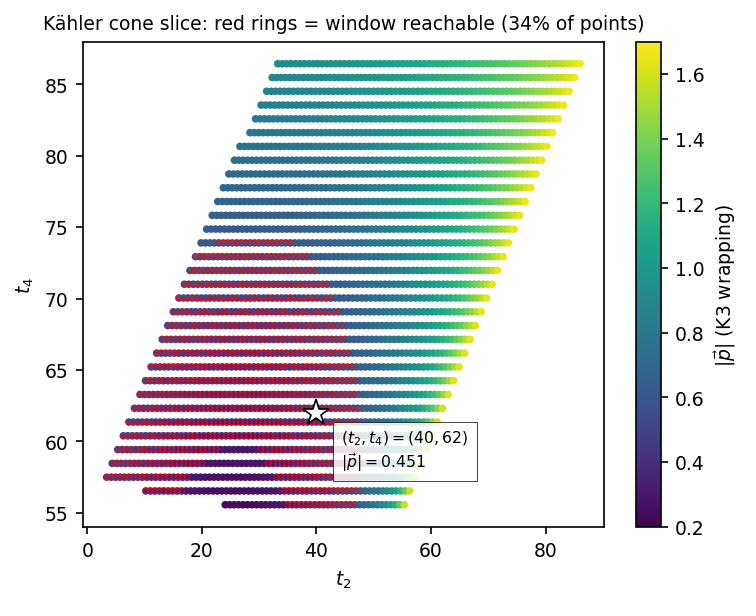
\includegraphics[width=.62\textwidth]{fig2_cone.png}
\caption{Slice of the K\"ahler cone in the $(t_2,t_4)$ plane at the LVS point. Colour is $|\vec p\,|$ for the K3 wrapping; red rings mark points from which the window is reachable.}\end{figure}
\paragraph{The window is a property of the family (the second calculation).} Computed directly on the orientifold database, on the three geometries sharing $(h^{2,1},\chi)=(81,-152)$, with the volume and \emph{both} diagonal del Pezzo divisors fixed and the K3 class wrapped, the window is reached in $13.2\%$, $17.0\%$ and $16.9\%$ of admissible points respectively --- the same order as the reference vacuum. Fourteen to sixteen thousand admissible points per geometry survive the positivity test, the bound $|\vec p|\leq|\vec w_{\rm geom}|=1.6956$ is saturated but never violated, and the three geometries return distinct distributions. \textbf{Reaching the window is therefore not a property of one member but of the family.} We record that this setup fixes both del Pezzo divisors whereas the reference calculation fixed one del Pezzo and the Wilson divisor: the genericities are comparable, the individual values are not. A further reserve: the database involution exchanges the two diagonal del Pezzo divisors, so only their sum survives the projection; the statistics above should be recomputed in the orientifold-even basis. The flat subspace remains two-dimensional, so the sum rule is untouched.\\[2pt]
Two robustness results: $|\vec p|$ is \emph{strictly invariant} over twelve orders of volume ($\mathcal V=10^6$ to $10^{18}$) and unchanged when $\tau_s/\mathcal V^{2/3}$ varies from $10^{-10}$ to $8.64\times10^{-12}$ --- the projections are a property of the direction in the flat subspace, not of the scale. They do depend on the position along the flat directions: $|\vec p|$(K3) runs from $0.337$ to $0.835$ across the cone.

\section{Routes 1--4: statistical and dynamical closure}
\paragraph{Route 1 --- family statistics.} Evaluated on the enumerated family with the Large-Volume hierarchy imposed, the sample splits \emph{cleanly in two}. Nine geometries converge --- those whose fibration is proper --- with median couplings $0.2964$, $0.3701$, $0.3760$, $0.4237$, $0.4608$, $0.4859$, $0.5220$, $0.5592$, $0.5771$; \textbf{eight of the nine lie inside the window} $[0.30,0.61]$, the ninth missing its lower edge by $0.004$. The eleven non-convergent geometries return medians from $0.667$ to $1.6956$, the latter being the ceiling $|\vec w_{\rm geom}|$ itself. \textbf{The two groups do not overlap.} Reaching the window is therefore not a matter of degree but a property of a subclass selected by the fibration. The first quartile of the convergent group is $0.376$; we record it as a quartile and not as a bound, since the smallest observed value lies below it. \textit{[Candidate, class property]}
\paragraph{Route 2 --- heterotic dual.} The $K3\times T^2$ dual matches the count ($n_V=5$ giving $S,T,U$ plus two Wilson lines; $n_H=82$), but the worldsheet computation does not fix the position along the flat directions. The route is closed as a derivation and retained as a long-term programme.
\paragraph{Route 3 --- full loop potential.} With the complete Kaluza--Klein and winding expressions over all twenty-five modulus pairs, the minimum sits on the cone boundary at $(t_2,t_4)=(84.96,85.46)$, where $t_2\simeq t_4$ and $|\vec p|=1.667$ --- far from the window.
\paragraph{Route 4 --- published functional form.} On $712$ cone points and $600$ coefficient draws, interior minima occur in $2.2\%$ of cases and never for positive winding coefficients, with median $|\vec p|=1.05$ and $7.7\%$ inside the window.
\paragraph{Synthesis.} No route fixes the position, and all confirm that the minimum tends to the boundary. \textbf{What Route~1 adds is that the position need not be fixed for the class statement to hold}: the convergent subclass reaches the window and the rest does not, with no overlap between them.

\section{Where the calculation stops, and why}
That position is fixed by the loop potential, and this is where the calculation stops. Three explicit attempts on this geometry all place the minimum on the cone boundary: a simplified form with only decreasing terms; the full expression restricted to three modulus pairs ($262$ of $1600$ grid points valid); and the full expression over all twenty-five pairs with $C^{KK}=(1,1,1,1,1)$ ($714$ of $1600$ valid), whose minimum sits at $(t_2,t_4)=(84.96,85.46)$ on the upper edge where $t_2\simeq t_4$, giving $|\vec p|(\mathrm{K3})=1.667$, far from the window. The uniform choice is not physical --- the coefficients depend on the brane configuration, the O3 loci for $\sigma_7$ lying on triple intersections --- so this is not a verdict on the geometry.

\emph{(An earlier version of this analysis quantified the same behaviour with a linear proxy $\sum_iC_i^2\tau_i$ for the Kaluza--Klein term and reported an interior minimum in $18\%$ of coefficient draws. That proxy is not the correct form; see below.)}

\textbf{The obstruction is not local to this construction.} The coefficients $C^{KK}$ and $C^W$ are not computable for a general Calabi--Yau: they have been obtained explicitly only for toroidal orientifolds~\cite{BHP}, while for Calabi--Yau compactifications the literature establishes the \emph{scaling} of the corrections with order-unity coefficients left as parameters~\cite{CCQ}. The entire fibre-inflation programme operates this way. \textbf{Hence $c_b$ cannot be fixed to a number today for this class of vacua, by anyone.}

\paragraph{The functional form, however, is known --- and it is unfavourable here.} The scan of the Kreuzer--Skarke database that produced this candidate~\cite{Shukla} also writes the loop potential explicitly for this class of geometry. The Kaluza--Klein piece is not a linear form in the four-cycle volumes but
\begin{equation}
\delta V_{KK}=\frac{\kappa|W_0|^2}{\mathcal V^2}\sum_\alpha(g_sC^{KK}_\alpha)^2\,\mathcal G_{\alpha\alpha},
\qquad
\mathcal G_{\alpha\beta}=\frac{1}{4\mathcal V^2}\big(2t^\alpha t^\beta-4\mathcal V k^{\alpha\beta}\big),
\end{equation}
with $k^{\alpha\beta}$ the inverse of $k_{\alpha\beta}=\kappa_{\alpha\beta\gamma}t^\gamma$, accompanied by a winding piece $-2\kappa|W_0|^2\mathcal V^{-3}\sum_\alpha C^W_\alpha/t^\alpha_\cap$ over the curves at the intersection loci. \textbf{We record that an earlier version of this analysis used a linear proxy $\sum_iC_i^2\tau_i$ for the first term and reported a threshold on a single coefficient ratio. That threshold was an artefact of the proxy and is withdrawn.}

Applied to this candidate with the correct forms, on a grid of $712$ points of the K\"ahler cone and $600$ coefficient draws, an interior minimum of the loop potential in the two-dimensional flat subspace occurs in $2.2\%$ of cases when the winding coefficients are allowed both signs, and \emph{never} when they are taken positive; at those interior minima the median is $|\vec p|=1.05$, and $7.7\%$ fall inside the window. \textbf{The corrected treatment is therefore less favourable than the one it replaces, not more.} The minimum tends to the boundary of the cone --- a behaviour the same reference notes as a known difficulty of this class, where the constraint $\tau_{\rm fibre}<\mathcal V^{2/3}$ is described as strong.

We also record that the natural route to fixing the coefficients does not work: the loop-correction systematics fixes the \emph{volume dependence} of the corrections, not their coefficients, and the $\mathcal N=2$ sub-sector enters only as a cut-off~\cite{CCQ}. They remain $O(1)$ and free.

\paragraph{But the angle does not survive into the observable.} The flat subspace is two-dimensional, so it carries \emph{two} light eigenstates, not one, and the mixing angle only decides how they share the coupling:
\begin{equation}
c_b=|\cos t\,p_1+\sin t\,p_2|,\qquad c_b'=|-\sin t\,p_1+\cos t\,p_2|
\qquad\Longrightarrow\qquad
\boxed{\;c_b^{2}+c_b'^{2}=p_1^{2}+p_2^{2}=|\vec p\,|^{2}.\;}
\end{equation}
The sum is the norm of a vector under a rotation, and the angle \emph{is} that rotation; the identity is exact, and it holds whatever the loop coefficients turn out to be (verified numerically at six arbitrary angles, constant to one part in $10^{10}$).

This matters because no experiment separates the two states. Each carries its own tower, $m_n^2=m_0^2+E_n^2$, and the flat directions lifted by loops have $m_0\simeq2.3\times10^{-3}$~meV against $E_1=24$~meV; varying $m_0$ by a factor three between the two states shifts their towers by $3.7\times10^{-8}$ in relative mass, six orders below the mass resolution of a torsion balance. \textbf{A fifth-force experiment therefore does not see two Yukawa terms but one, of strength $\alpha_b^2+\alpha_b'^2$ --- precisely the angle-independent quantity.} At the reference point this gives, with no loop coefficient whatever,
\begin{equation}
\alpha_b^2+\alpha_b'^2=2w_1|\vec p\,|^2=2.24 .
\end{equation}

The unknown that remains is the \emph{position} along the flat directions, which fixes $|\vec p\,|$ and still varies from $0.26$ to $1.65$ across the cone --- whence a candidate-specific bound $c_b\leq1.651$, $29\%$ tighter than the general one. But its status changes: a measurement of $\alpha_b^2+\alpha_b'^2$ returns $|\vec p\,|^2$ and hence selects the position, without passing through the loop coefficients. \textbf{Finding the vacuum ceases to be a prerequisite for the prediction and becomes a consequence of the measurement.} We record the physical price plainly: this framework contains \emph{two} light dark scalars, not one. Their towers being indistinguishable, no result of the parent series is falsified by this --- but the radiation budget must be counted with two towers.

What is stated instead is conditional and falsifiable:
\begin{quote}\emph{The angle-independent combination $\alpha_b^2+\alpha_b'^2=2w_1|\vec p\,|^2$ is fixed by the geometry once the position in the K\"ahler cone is given, and requires no loop coefficient. That position is not fixed by the loop potential on this candidate: with the published functional form the minimum tends to the cone boundary, and interior minima --- rare, and mostly outside the window --- carry $|\vec p|$ between $0.46$ and $1.54$. The candidate is therefore not excluded and not confirmed. What a measurement of $\alpha_b^2+\alpha_b'^2$ would do is select the position directly.}\end{quote}

\section{The normalisation chain, closed}
Each arrow of the reduction carries an explicit factor, and the two Einstein-frame conditions are exact:
\begin{center}\small
\begin{tabular}{clc}\toprule
step & content & check\\\midrule
1 & $10\to9$ on the interval: $\alpha_1=1/4\sqrt7$, $\beta_1=-\sqrt7/4$ & $7\alpha_1+\beta_1=0$ exactly\\
2 & $9\to4$ on $X_5$: $\alpha_2=\sqrt{5/28}$, $\beta_2=-1/\sqrt{35}$ & $2\alpha_2+5\beta_2=0$ exactly\\
3 & D8 DBI: dilaton weight $(p-3)/2\sqrt2$, geometric $9\alpha_1$ and $4\alpha_2+5\beta_2$, $\times\sqrt2$ & $|\vec w|^2=6$\\
4 & projection on the light modulus: $c_b=|\hat n\cdot\vec w|$ & $\leq\sqrt{255/56}=2.1339$\\
5 & $5\to4$: $w_1=u|\psi_1(0)|^2=4.43\times1.24153=5.5000$ & $\alpha_b=3.3166\,c_b$\\
6 & closure against the parent's $\alpha_b=3.3\,c_b$ & agreement to $0.50\%$\\\bottomrule
\end{tabular}
\end{center}
At the candidate, $c_b=0.4514$ gives $\alpha_b=1.4971$, and the sum rule $\sqrt{2w_1|\vec p|^2}$ returns $1.4971$: the two routes to the observable agree identically. The only link not closed is step~4, the projection, which depends on the position in the cone --- and step~5 read through the sum rule bypasses it.

\section{What this paper does not claim}
It does not claim that $c_b$ is derived. It exhibits a candidate on which the coupling \emph{can} reach the window, shows that this is a property of a fibration-selected subclass rather than an accident, and identifies the one quantity --- the position along the flat directions --- that would fix it and that no present calculation fixes. The angle-independent sum rule makes the observable insensitive to that position's \emph{partner}, the mixing angle, but not to the position itself. \textbf{A reader who takes away ``$c_b=0.45$ from string theory'' has misread this paper; one who takes away ``the window is reachable, on an enumerated class, for a reason the geometry supplies, and the remaining freedom is one measurable number'' has read it correctly.}

\section{How this paper dies}
\emph{(i)} If the loop coefficients of this class are ever computed and place the minimum away from $|\vec p|\in[0.30,0.61]$ at every interior point of the cone, this candidate is excluded; if they place it inside, the conditional becomes a value. \emph{(ii)} If $|\vec w|^2=6$ is found already published, that claim is withdrawn and the rest stands. \emph{(iii)} If the hidden sector on the far wall overshoots the radiation budget, the symmetric Type I$'$ configuration --- the only one compatible with $F_0=0$ --- is excluded, and this embedding with it. \emph{(iv)} If the torsion balance reaches Yukawa strength $8/3$ at $8.2\,\mu$m and finds Newton, the parent framework dies and this paper with it. \emph{(v)} If a sharper determination of the ultraviolet cutoff or of the LVS anti-de Sitter depth tips the domain wall bound of \S5.1 --- satisfied here by only a factor $15$ on the gravitino side --- the reference vacuum is excluded. \emph{(vi)} If a warped realisation is constructed --- the only known escape from the interval-length problem --- the unwarped reduction used throughout must be redone.

\paragraph{Superseded values.} For traceability we record the numbers that earlier stages of this work produced and that are now withdrawn: $|\vec p|=0.7023$ and $0.6283$ for the Wilson wrapping and $0.307$ for the K3, all computed at points outside the K\"ahler cone or with the metric taken in the two-cycle basis, and one dP7 value discarded as a numerical artefact of the degenerate locus $t_2=t_4$. None of them should be quoted.

\paragraph{Reproducibility.} Every number above is produced by \texttt{02\_calculs/repro.py} and stored in \texttt{06\_preuves/*.json}; the technical worksheet \texttt{00\_cible/FEUILLE\_TECHNIQUE.md} lists the conventions, the pitfalls encountered and the checks that must precede each step; all figures are regenerated by \texttt{02\_calculs/figures.py}.


% ═══════════════════════════════════════════════════════════════════════════
%  APPENDICE DE LIAISON — identique dans les sept articles.
%  % ═══════════════════════════════════════════════════════════════════════════
%  APPENDICE DE LIAISON — identique dans les sept articles.
%  % ═══════════════════════════════════════════════════════════════════════════
%  APPENDICE DE LIAISON — identique dans les sept articles.
%  \input{appendix-where} juste avant \begin{thebibliography} ou la biblio.
%  Il répond à : qui vit où, et qu'est-ce que la série a changé en cours de route.
% ═══════════════════════════════════════════════════════════════════════════
\section*{Appendix: which sector lives where, and what changed}
\addcontentsline{toc}{section}{Appendix: which sector lives where}

The series was written over several months and \textbf{two of its assignments moved}.
A reader who meets the articles out of order is owed an explicit map rather than an
inference, so it is given here, identically in all seven papers.

\subsection*{A.1 The three locations}
The geometry has three places where physics can sit: the \emph{brane} at $y=0$,
the \emph{bulk} of the $8.2\,\mu$m interval, and the \emph{far wall} at $y=\pi R$.
\begin{center}\small
\begin{tabular}{llll}\toprule
sector & lives on & carried by & established in\\\midrule
ordinary matter & \textbf{brane} & thin core, Standard Model & I\\
gravity, radion, graviton & \textbf{bulk} & five-dimensional fields & I\\
the mediator $\Phi$ and its tower & \textbf{bulk} & Airy states of the $|y|$ well & II\\
the galactic response & \textbf{bulk} $\to$ brane & $\Phi$ exchange between baryons & III\\
dark matter & \textbf{see A.2} & --- & III, revisited in VI\\
dark energy & \textbf{see A.3} & --- & III, revisited in VI\\
hidden gauge sector & \textbf{far wall} & eight D8 and one O8 & V\\\bottomrule
\end{tabular}
\end{center}

\subsection*{A.2 Dark matter: the reservoir, and what the wall reading adds}
Articles~I--IV place dark matter in the \emph{bulk}: the excited states of the Airy
tower, populated cold at birth, collisionless, carrying at least $98.6\%$ of the dark
sector's density. That assignment does the work in three places. It makes structure
formation identical to cold dark matter at linear order. It answers the Bullet Cluster
by mass budget alone --- cluster masses are cluster masses, and the lensing tracks the
reservoir, which is why the lensing--dynamics difficulty of purely modified dynamics is
not inherited. And it fixes the radiation budget of Article~I.

Article~VI proposes a different reading: dark matter as the ordinary matter of the six
other regions of the same wall, seen through the bulk, giving
$\Omega_{\rm DM}/\Omega_b=N_{\rm regions}-1=6$ against an observed $5.31$.
\textbf{These are not the same statement, and we do not pretend otherwise.}

What they share is everything the phenomenology uses: in both readings the dark
component is cold, collisionless, and carries the mass, so lensing, the Bullet Cluster
and linear structure formation are unaffected. What differs is the \emph{constituent}:
quanta of $\Phi$ in the first, baryons of other regions in the second.
\textbf{The two are compatible if the tower reservoir is not required to be the whole
of the dark matter} --- and Article~III's own argument only requires it to dominate the
budget, not to be exhaustive. \Open

\subsection*{A.3 Dark energy: a bulk scalar, then a brane curvature}
Articles~I--IV treat $\Phi$ as the dark-energy candidate --- a bulk scalar engine. That
attempt \emph{failed by forty orders of magnitude}: a four-dimensional scalar cannot
reach $2.4$~meV from a $10^{-13}$~eV engine scale. The failure is recorded, not hidden.

Article~VI relocates dark energy \emph{to the brane}, as the extrinsic curvature of the
D8 wall in the cosmological bulk, $\Lambda_4=\varepsilon^2(1/R)^4$ with
$\varepsilon\simeq10^{-2}$. The mechanism supplies $(1/R)^4$ outright and leaves a gap
of $10^4$ rather than $10^{40}$. \textbf{$\Phi$ is correspondingly demoted from
dark-energy candidate to dark-sector mediator}, which is the role Articles~II and III
already gave it in every equation they actually use. \Candidate, declared tuning.

\subsection*{A.4 The radial acceleration relation, and what makes galaxies turn}
The relation is the one place where brane and bulk are \emph{both} indispensable, and
where nothing has moved since Article~III.

Baryons sit on the brane. They source $\Phi$, which propagates in the bulk with mass
$m_\Phi=24$~meV and hence Compton range $8.2\,\mu$m --- microscopic, so no fifth force
acts between laboratory bodies. What acts at galactic scale is not the free field but
the \emph{medium}: the coherent component of the dark sector responds to the baryonic
distribution, and that response, read back on the brane, is the extra acceleration.
The response saturates, which is why it produces a relation --- an acceleration scale
$g_\dagger$ --- rather than a rescaling of Newton's constant.

Three consequences, all in Article~III and unchanged:
\begin{itemize}\itemsep2pt
\item the response couples to the trace $T^\mu_{\ \mu}$, hence to mass and not to
      composition; the universality is bounded on 171 SPARC galaxies;
\item the response is carried by at most $1.4\%$ of the dark sector, the coherent part,
      so it never competes with the reservoir in the mass budget --- \textbf{galaxies
      turn because of the medium, they weigh because of the reservoir};
\item the response \emph{dies} in weak field, which is the ultra-diffuse galaxy test,
      and it dies in a decoherence bubble around the Sun, which is why Cassini is
      satisfied identically rather than by tuning.
\end{itemize}
\textbf{Neither relocation of A.2 or A.3 touches this.} The galactic response was never
assigned to the dark-energy sector, and it is not the reservoir either; it is the third
role, and it is the one the framework was built to explain.

\subsection*{A.5 What a reader should carry between articles}
Articles~I--IV stand on their own evidence and are not modified by V--VII: no result of
theirs is derived from the string embedding, and the embedding cannot promote any of
their labels. What V--VII add is an ultraviolet origin for one constant, a candidate
geometry, and two consequences of that geometry. What they \emph{change} is recorded
above and nowhere else: two relocations, both declared, neither retroactive.
 juste avant \begin{thebibliography} ou la biblio.
%  Il répond à : qui vit où, et qu'est-ce que la série a changé en cours de route.
% ═══════════════════════════════════════════════════════════════════════════
\section*{Appendix: which sector lives where, and what changed}
\addcontentsline{toc}{section}{Appendix: which sector lives where}

The series was written over several months and \textbf{two of its assignments moved}.
A reader who meets the articles out of order is owed an explicit map rather than an
inference, so it is given here, identically in all seven papers.

\subsection*{A.1 The three locations}
The geometry has three places where physics can sit: the \emph{brane} at $y=0$,
the \emph{bulk} of the $8.2\,\mu$m interval, and the \emph{far wall} at $y=\pi R$.
\begin{center}\small
\begin{tabular}{llll}\toprule
sector & lives on & carried by & established in\\\midrule
ordinary matter & \textbf{brane} & thin core, Standard Model & I\\
gravity, radion, graviton & \textbf{bulk} & five-dimensional fields & I\\
the mediator $\Phi$ and its tower & \textbf{bulk} & Airy states of the $|y|$ well & II\\
the galactic response & \textbf{bulk} $\to$ brane & $\Phi$ exchange between baryons & III\\
dark matter & \textbf{see A.2} & --- & III, revisited in VI\\
dark energy & \textbf{see A.3} & --- & III, revisited in VI\\
hidden gauge sector & \textbf{far wall} & eight D8 and one O8 & V\\\bottomrule
\end{tabular}
\end{center}

\subsection*{A.2 Dark matter: the reservoir, and what the wall reading adds}
Articles~I--IV place dark matter in the \emph{bulk}: the excited states of the Airy
tower, populated cold at birth, collisionless, carrying at least $98.6\%$ of the dark
sector's density. That assignment does the work in three places. It makes structure
formation identical to cold dark matter at linear order. It answers the Bullet Cluster
by mass budget alone --- cluster masses are cluster masses, and the lensing tracks the
reservoir, which is why the lensing--dynamics difficulty of purely modified dynamics is
not inherited. And it fixes the radiation budget of Article~I.

Article~VI proposes a different reading: dark matter as the ordinary matter of the six
other regions of the same wall, seen through the bulk, giving
$\Omega_{\rm DM}/\Omega_b=N_{\rm regions}-1=6$ against an observed $5.31$.
\textbf{These are not the same statement, and we do not pretend otherwise.}

What they share is everything the phenomenology uses: in both readings the dark
component is cold, collisionless, and carries the mass, so lensing, the Bullet Cluster
and linear structure formation are unaffected. What differs is the \emph{constituent}:
quanta of $\Phi$ in the first, baryons of other regions in the second.
\textbf{The two are compatible if the tower reservoir is not required to be the whole
of the dark matter} --- and Article~III's own argument only requires it to dominate the
budget, not to be exhaustive. \Open

\subsection*{A.3 Dark energy: a bulk scalar, then a brane curvature}
Articles~I--IV treat $\Phi$ as the dark-energy candidate --- a bulk scalar engine. That
attempt \emph{failed by forty orders of magnitude}: a four-dimensional scalar cannot
reach $2.4$~meV from a $10^{-13}$~eV engine scale. The failure is recorded, not hidden.

Article~VI relocates dark energy \emph{to the brane}, as the extrinsic curvature of the
D8 wall in the cosmological bulk, $\Lambda_4=\varepsilon^2(1/R)^4$ with
$\varepsilon\simeq10^{-2}$. The mechanism supplies $(1/R)^4$ outright and leaves a gap
of $10^4$ rather than $10^{40}$. \textbf{$\Phi$ is correspondingly demoted from
dark-energy candidate to dark-sector mediator}, which is the role Articles~II and III
already gave it in every equation they actually use. \Candidate, declared tuning.

\subsection*{A.4 The radial acceleration relation, and what makes galaxies turn}
The relation is the one place where brane and bulk are \emph{both} indispensable, and
where nothing has moved since Article~III.

Baryons sit on the brane. They source $\Phi$, which propagates in the bulk with mass
$m_\Phi=24$~meV and hence Compton range $8.2\,\mu$m --- microscopic, so no fifth force
acts between laboratory bodies. What acts at galactic scale is not the free field but
the \emph{medium}: the coherent component of the dark sector responds to the baryonic
distribution, and that response, read back on the brane, is the extra acceleration.
The response saturates, which is why it produces a relation --- an acceleration scale
$g_\dagger$ --- rather than a rescaling of Newton's constant.

Three consequences, all in Article~III and unchanged:
\begin{itemize}\itemsep2pt
\item the response couples to the trace $T^\mu_{\ \mu}$, hence to mass and not to
      composition; the universality is bounded on 171 SPARC galaxies;
\item the response is carried by at most $1.4\%$ of the dark sector, the coherent part,
      so it never competes with the reservoir in the mass budget --- \textbf{galaxies
      turn because of the medium, they weigh because of the reservoir};
\item the response \emph{dies} in weak field, which is the ultra-diffuse galaxy test,
      and it dies in a decoherence bubble around the Sun, which is why Cassini is
      satisfied identically rather than by tuning.
\end{itemize}
\textbf{Neither relocation of A.2 or A.3 touches this.} The galactic response was never
assigned to the dark-energy sector, and it is not the reservoir either; it is the third
role, and it is the one the framework was built to explain.

\subsection*{A.5 What a reader should carry between articles}
Articles~I--IV stand on their own evidence and are not modified by V--VII: no result of
theirs is derived from the string embedding, and the embedding cannot promote any of
their labels. What V--VII add is an ultraviolet origin for one constant, a candidate
geometry, and two consequences of that geometry. What they \emph{change} is recorded
above and nowhere else: two relocations, both declared, neither retroactive.
 juste avant \begin{thebibliography} ou la biblio.
%  Il répond à : qui vit où, et qu'est-ce que la série a changé en cours de route.
% ═══════════════════════════════════════════════════════════════════════════
\section*{Appendix: which sector lives where, and what changed}
\addcontentsline{toc}{section}{Appendix: which sector lives where}

The series was written over several months and \textbf{two of its assignments moved}.
A reader who meets the articles out of order is owed an explicit map rather than an
inference, so it is given here, identically in all seven papers.

\subsection*{A.1 The three locations}
The geometry has three places where physics can sit: the \emph{brane} at $y=0$,
the \emph{bulk} of the $8.2\,\mu$m interval, and the \emph{far wall} at $y=\pi R$.
\begin{center}\small
\begin{tabular}{llll}\toprule
sector & lives on & carried by & established in\\\midrule
ordinary matter & \textbf{brane} & thin core, Standard Model & I\\
gravity, radion, graviton & \textbf{bulk} & five-dimensional fields & I\\
the mediator $\Phi$ and its tower & \textbf{bulk} & Airy states of the $|y|$ well & II\\
the galactic response & \textbf{bulk} $\to$ brane & $\Phi$ exchange between baryons & III\\
dark matter & \textbf{see A.2} & --- & III, revisited in VI\\
dark energy & \textbf{see A.3} & --- & III, revisited in VI\\
hidden gauge sector & \textbf{far wall} & eight D8 and one O8 & V\\\bottomrule
\end{tabular}
\end{center}

\subsection*{A.2 Dark matter: the reservoir, and what the wall reading adds}
Articles~I--IV place dark matter in the \emph{bulk}: the excited states of the Airy
tower, populated cold at birth, collisionless, carrying at least $98.6\%$ of the dark
sector's density. That assignment does the work in three places. It makes structure
formation identical to cold dark matter at linear order. It answers the Bullet Cluster
by mass budget alone --- cluster masses are cluster masses, and the lensing tracks the
reservoir, which is why the lensing--dynamics difficulty of purely modified dynamics is
not inherited. And it fixes the radiation budget of Article~I.

Article~VI proposes a different reading: dark matter as the ordinary matter of the six
other regions of the same wall, seen through the bulk, giving
$\Omega_{\rm DM}/\Omega_b=N_{\rm regions}-1=6$ against an observed $5.31$.
\textbf{These are not the same statement, and we do not pretend otherwise.}

What they share is everything the phenomenology uses: in both readings the dark
component is cold, collisionless, and carries the mass, so lensing, the Bullet Cluster
and linear structure formation are unaffected. What differs is the \emph{constituent}:
quanta of $\Phi$ in the first, baryons of other regions in the second.
\textbf{The two are compatible if the tower reservoir is not required to be the whole
of the dark matter} --- and Article~III's own argument only requires it to dominate the
budget, not to be exhaustive. \Open

\subsection*{A.3 Dark energy: a bulk scalar, then a brane curvature}
Articles~I--IV treat $\Phi$ as the dark-energy candidate --- a bulk scalar engine. That
attempt \emph{failed by forty orders of magnitude}: a four-dimensional scalar cannot
reach $2.4$~meV from a $10^{-13}$~eV engine scale. The failure is recorded, not hidden.

Article~VI relocates dark energy \emph{to the brane}, as the extrinsic curvature of the
D8 wall in the cosmological bulk, $\Lambda_4=\varepsilon^2(1/R)^4$ with
$\varepsilon\simeq10^{-2}$. The mechanism supplies $(1/R)^4$ outright and leaves a gap
of $10^4$ rather than $10^{40}$. \textbf{$\Phi$ is correspondingly demoted from
dark-energy candidate to dark-sector mediator}, which is the role Articles~II and III
already gave it in every equation they actually use. \Candidate, declared tuning.

\subsection*{A.4 The radial acceleration relation, and what makes galaxies turn}
The relation is the one place where brane and bulk are \emph{both} indispensable, and
where nothing has moved since Article~III.

Baryons sit on the brane. They source $\Phi$, which propagates in the bulk with mass
$m_\Phi=24$~meV and hence Compton range $8.2\,\mu$m --- microscopic, so no fifth force
acts between laboratory bodies. What acts at galactic scale is not the free field but
the \emph{medium}: the coherent component of the dark sector responds to the baryonic
distribution, and that response, read back on the brane, is the extra acceleration.
The response saturates, which is why it produces a relation --- an acceleration scale
$g_\dagger$ --- rather than a rescaling of Newton's constant.

Three consequences, all in Article~III and unchanged:
\begin{itemize}\itemsep2pt
\item the response couples to the trace $T^\mu_{\ \mu}$, hence to mass and not to
      composition; the universality is bounded on 171 SPARC galaxies;
\item the response is carried by at most $1.4\%$ of the dark sector, the coherent part,
      so it never competes with the reservoir in the mass budget --- \textbf{galaxies
      turn because of the medium, they weigh because of the reservoir};
\item the response \emph{dies} in weak field, which is the ultra-diffuse galaxy test,
      and it dies in a decoherence bubble around the Sun, which is why Cassini is
      satisfied identically rather than by tuning.
\end{itemize}
\textbf{Neither relocation of A.2 or A.3 touches this.} The galactic response was never
assigned to the dark-energy sector, and it is not the reservoir either; it is the third
role, and it is the one the framework was built to explain.

\subsection*{A.5 What a reader should carry between articles}
Articles~I--IV stand on their own evidence and are not modified by V--VII: no result of
theirs is derived from the string embedding, and the embedding cannot promote any of
their labels. What V--VII add is an ultraviolet origin for one constant, a candidate
geometry, and two consequences of that geometry. What they \emph{change} is recorded
above and nowhere else: two relocations, both declared, neither retroactive.

\toolsstatement
\traceability{5}{The norm identities, the bound, the reference vacuum, the family statistics and the sum rule are produced by \texttt{scripts/repro.py}; the figures by \texttt{scripts/figures.py}.}
\bibliographystyle{unsrt}\bibliography{ddf-refs}
\end{document}
